\documentclass[11pt]{article}

\usepackage{amsmath}
\usepackage{amssymb}
\usepackage{fancyhdr}
\usepackage[total={6in, 9in}, headheight=53pt]{geometry}
\usepackage{graphicx}
\usepackage[utf8]{inputenc}
\usepackage{tikz}

\renewcommand{\familydefault}{\sfdefault}

\pagestyle{fancy}
\lhead{\nouppercase{\leftmark}}
\rhead{\rightmark}

\begin{document}

\begin{center}

\includegraphics[width=0.5\textwidth]{adjoint.png}

\textbf{\LARGE ADJOINT UK LTD}

\vspace{0.5cm}

\hrule

\vspace{1.5cm}

\textbf{\Large INDUSTRIAL PLACEMENT 2019}

\vspace{0.5cm}

\textbf{\Large PLACEMENT REPORT}

\vspace{1.5cm}

{\large \textbf{STUDENT:} DAVID KURNIADI ANGDINATA}

\vspace{0.5cm}

{\large \textbf{DEGREE:} MENG MATHEMATICS AND COMPUTER SCIENCE FOUR}

\vspace{0.5cm}

{\large \textbf{TUTOR:} NICOLAS WU}

\vspace{1.5cm}

{\small \textbf{MANAGER:} \hspace{3cm}}

\vspace{0.5cm}

{\small \textbf{EMAIL:} \hspace{3cm}}

\vspace{0.5cm}

{\small \textbf{SIGNATURE:} \hspace{3cm}}

\vspace{0.5cm}

{\small \textbf{DATE:} \hspace{3cm}}

\end{center}

\pagebreak

\section{Introduction}

\subsection{Company profile}

\emph{Adjoint} UK Ltd. \cite{adjoint} is a private independent software company in the financial technology sector based in central London. Founded in 2016 by Stephen Diehl, Havell Rodrigues, and Darren Tseng in Boston, it has since expanded to several cities across three countries.

Adjoint aims to build modern software solutions for intercompany financial workflow automation and virtual account management, to simplify and control enterprise processes to give global cash transparency. Its main products and technologies include \emph{Treasury} \cite{treasury}, an intuitive yet powerful real-time payment and settlement platform for corporate treasury, and \emph{Uplink} \cite{uplink}, a next-generation distributed ledger database for secure multiparty computation written in a carefully designed runtime \emph{FCL} \cite{fcl}, which is in turn written in the functional language \emph{Haskell}.

\begin{center}
\includegraphics[width=\textwidth]{uplink.png}
\end{center}

Adjoint's technologies provide a strong transaction privacy for all participating and public parties, while allowing any party to receive reliable answers to its queries \cite{cryptography}. To ensure this security, several cryptographic systems are developed and deployed internally over the years to suit specific requirements of each solution. Some of these have been made open source and have accepted community contributions, including a Haskell library on \emph{Bulletproofs} \cite{bulletproofs}, short non-interactive zero-knowledge proof systems that require no trusted setup.

\subsection{Organisation roles}

The main development team in Adjoint consists of the \emph{product team} and the \emph{core team}, the former of which focuses on the front-end development of directly marketable products like Treasury, while the latter focuses on the workings behind the FCL language and the cryptographic roadmap. In particular, the core team aims to develop and maintain the syntax, semantics, usability, and performance of the FCL language, as well as a multitude of primitives and protocols that together constitute the cryptographic roadmap.

My role in Adjoint is to develop and maintain the existing cryptography stack as a cryptography engineer in the core team. My job description involves developing secure communication protocols using zero-knowledge proofs, as well as directing and overseeing the cryptographic roadmap, both of which involve tight collaboration with a colleague. Most immediate design decisions are made as a five-man team, but long-term software development ideas are carefully thought through, through frequent communication with the chief technology officer (CTO).

\pagebreak

\section{Projects}

Adjoint's cryptographic roadmap is a tree of several modular libraries, some of which are publicly available as repositories in its GitHub landing page. Each of these serves as an implementation for a particular cryptographic primitive, such as hash functions and bilinear pairings, or a particular cryptographic protocol, such as key exchanges and zero-knowledge proofs.

\begin{center}
\includegraphics[width=\textwidth]{github.png}
\end{center}

While most cryptosystems are developed in low-level languages like \emph{C} for optimal computation speeds, Adjoint aims to produce highly sound and comprehensible code, using the functional \emph{Haskell} as its main development language. Although this may compromise performance, most protocols have computation times in the millisecond range and are relatively unnoticeable.

In the following sections, I will detail the various libraries I have developed or contributed over the summer, in a roughly chronological order unless specified otherwise.

\subsection{The library for the FCL language}

Before delving into cryptography, my first task was to explore the FCL language and suggest possible improvements. I was lead to the problem that \emph{reachability checking} of certain graph-theoretic structures in the language, known as \emph{Petri nets}, had a time complexity factorial over the number of nodes. I did some domain research afterwards and came up with several solutions.

Initially, I tried a \emph{linear programming} approach based on the ideas in several papers \cite{kostin}, but quickly realised its domain-specific limitations, such as being unable to check other equally important graph-theoretic conditions in the FCL Petri net construction and produce user-friendly errors upon failure. The other solution I tried was a \emph{graph unfolding} approach through \emph{McMillan's algorithm} \cite{mcmillan}, which does not have this limitation but was somewhat elaborate in its construction, and as such was only partially implemented by the end of the week.

A colleague continued from where I stopped, working along the same lines to improve the FCL language, and developed the ideas further as part of a much larger project. As such, I was able to frequently discuss design decisions throughout the project over twelve weeks, with the final product being a highly flexible prototype that avoided reachability checking completely.

\subsection{The library for pairing-based cryptographic protocols}

My primary task was to develop and maintain the \emph{pairing-based elliptic-curve cryptography} (PBECC) roadmap. This included \emph{bilinear pairings} and \emph{arithmetic circuits} as primitives, which were used to implement various protocols based on the modern concept of \emph{zero-knowledge succinct non-interactive arguments of knowledge (zk-SNARKs)}. These are protocols that allow a party to prove to another, succinctly and without any interaction, that they possess the knowledge of certain information, without conveying any other information apart from this fact.

Upon quickly familiarising myself with the relevant theory and the existing cryptographic stack, I was tasked to implement a protocol based on an instrumental 2016 paper by Jen Groth \cite{groth}, having the existing \emph{Sonic} protocol \cite{sonic} implementation as a background example. The dependency graph of the PBECC stack would subsequently look like the following.
\begin{center}
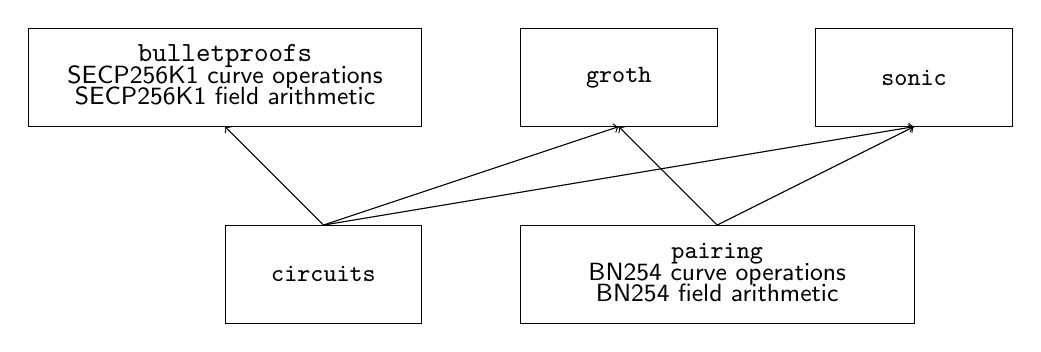
\begin{tikzpicture}[scale=1.25]
\draw (-3, 0) rectangle node{\small \texttt{circuits}} (-1, 1);
\draw [->] (-2, 1) to (-3, 2);
\draw [->] (-2, 1) to (1, 2);
\draw [->] (-2, 1) to (4, 2);
\draw (0, 0) rectangle node[above]{\small \texttt{pairing}} node{\small BN254 curve operations} node[below]{\small BN254 field arithmetic} (4, 1);
\draw [->] (2, 1) to (1, 2);
\draw [->] (2, 1) to (4, 2);
\draw (-5, 2) rectangle node[above]{\texttt{bulletproofs}} node{\small SECP256K1 curve operations} node[below]{\small SECP256K1 field arithmetic} (-1, 3);
\draw (0, 2) rectangle node{\small \texttt{groth}} (2, 3);
\draw (3, 2) rectangle node{\small \texttt{sonic}} (5, 3);
\end{tikzpicture}
\end{center}
Here \emph{SECP256K1} and \emph{BN254} are well-known elliptic curves, whose curve operations and field arithmetic had to be implemented internally or externally in their respective libraries.

While the exact details of the implementation will be omitted here for brevity, the protocol is a set of algorithms, taking \emph{quadratic arithmetic programs (QAPs)} \cite{qap} as inputs, and returning the relevant information without leakage. For instance, its \texttt{verify} algorithm takes, as input,
\begin{itemize}
\item a variable list of field elements $ a_0, \dots, a_l $ obtained from arithmetic circuits,
\item a fixed list of group elements $ \alpha g, \beta h, \gamma h, \dots $ computed by its \texttt{setup} algorithm, and
\item a \emph{proof} consisting of three group elements $ Ag, Bh, Cg $ computed by its \texttt{prove} algorithm.
\end{itemize}
Here $ g $ and $ h $ are generators of certain elliptic curves paired by a suitable function $ \langle -, - \rangle $, while the remaining computed constants are unknown elements of a Galois field, assuming the hardness of the \emph{discrete logarithm problem}. The verification algorithm then returns true whenever
$$ \langle Ag, Bh \rangle = \langle \alpha g, \beta h \rangle \cdot \langle \textstyle{\sum_{i = 0}^l} a_i\tfrac{\beta u_i(x) + \alpha v_i(x) + w_i(x)}{\gamma}g, \gamma h \rangle \cdot \langle Cg, \delta h \rangle. $$

These were admittedly far more laborious to write than it was conceptually difficult, as it only took two days to design the relevant data structures and produce a prototype with unit tests. Rather, the main issue was an elegant integration with existing QAPs, which had readily available \emph{QuickCheck} tests and \emph{Criterion} benchmarks, while my implementation made use of slightly different data structures. Unfortunately, there were no easy conversions between the two representations, so work was agreeably paused until further insight is shed.

It was only in my final week that I sought assistance from a colleague who was jointly tasked to implement this protocol over the summer. After much discussion, we managed to refactor the current implementation sufficiently to use the existing representation of QAPs, producing a workable prototype. Subsequently, we also ported the tests and benchmarks over, as well as the various improvements we made to primitive libraries over the past three months in the form of significant restructuring of the PBECC stack, to be detailed in the following sections.

\pagebreak

\subsection{An efficient library for Galois field arithmetic}

After the preliminary implementation of \texttt{groth} in the first month, there was evidently at least one unsatisfactory component to the overall structure of the PBECC stack, namely that the protocols dependent on \texttt{pairing} use the internal BN254 elliptic curve, which only slightly differs in parameters from the SECP256K1 elliptic curve in \texttt{bulletproofs} taken from an external library. This presents a slight duplication of algorithm code for group operations, which is acceptable, but it also induces a massive duplication of Galois field arithmetic code.

For instance, a single elliptic curve requires the arithmetic of at least two Galois fields. One of these would define the elliptic curve equation, and the other would be a Galois field of prime order used as scalars for multiplication, since the main subgroup of an elliptic curve has prime order to ensure security for cryptographic purposes. On the other hand, the Galois fields used in pairing-friendly elliptic curves are often made of three towers of simple extensions, requiring three further definitions for their arithmetic, and this was the case in \texttt{pairing}, as shown below.
\begin{center}
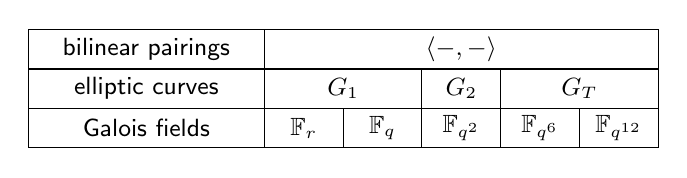
\begin{tikzpicture}[scale=0.5]
\draw (0, 0) rectangle (16, 3);
\draw (0, 2) rectangle node{\small bilinear pairings} (6, 3);
\draw (6, 2) rectangle node{\small $ \langle -, - \rangle $} (16, 3);
\draw (0, 1) rectangle node{\small elliptic curves} (6, 2);
\draw (6, 1) rectangle node{\small $ G_1 $} (10, 2);
\draw (10, 1) rectangle node{\small $ G_2 $} (12, 2);
\draw (12, 1) rectangle node{\small $ G_T $} (16, 2);
\draw (0, 0) rectangle node{\small Galois fields} (6, 1);
\draw (6, 0) rectangle node{\small $ \mathbb{F}_r $} (8, 1);
\draw (8, 0) rectangle node{\small $ \mathbb{F}_q $} (10, 1);
\draw (10, 0) rectangle node{\small $ \mathbb{F}_{q^2} $} (12, 1);
\draw (12, 0) rectangle node{\small $ \mathbb{F}_{q^6} $} (14, 1);
\draw (14, 0) rectangle node{\small $ \mathbb{F}_{q^{12}} $} (16, 1);
\end{tikzpicture}
\end{center}

While this was not time-critical, I was subsequently tasked to implement group operations on \emph{Edwards curves}, a family of elliptic curves that admit a \emph{complete} and \emph{stongly unified} addition formula, simplifying many algorithms and protecting against side-channel timing attacks. Specifically, the parameters of interest were that of the newly discovered \emph{Jubjub} curve \cite{jubjub} used in modern zk-SNARK constructions, whose arithmetic was unavailable in \texttt{pairing} or any external libraries. It was clear that massive code duplication is unavoidable at the current state.

I proposed a separation of concerns by developing an internal library dedicated to Galois field arithmetic, with firm foundations on results in basic algebra. This would serve as a mathematical abstraction over the Galois fields defined for existing SECP256K1 and BN254 curves, greatly reducing unnecessary code duplication in the bilinear and increasing overall robustness of the PBECC stack. This would also hasten the implementation of any future protocol requiring Galois field arithmetic, which are abundant by the finitary nature of cryptography.

Upon agreement with the CTO, I designed a \texttt{class GaloisField k} for general Galois fields, constrained by the usual constraints as well as \texttt{Fractional}. This would possess type class functions such as recovering its non-zero characteristic with \texttt{char :: k -> Natural}, recovering its embedding degree with \texttt{deg :: k -> Natural}, and computing \emph{Frobenius endomorphisms} efficiently with \texttt{frob :: k -> k}. Whilst \texttt{char} and \texttt{deg} could have been of type \texttt{Natural}, adding \texttt{k} would remove type parameter ambiguity.

I added a type for Galois fields of prime order, which had a unique prime characteristic that is encoded in the type-level with the \texttt{Nat} kind and not checked for primality.
\begin{verbatim}
    newtype Prime (p :: Nat) = P Natural
\end{verbatim}
The usual functions on \texttt{Fractional} were implemented with usual modular arithmetic, although there were much room for optimisations, such as using \texttt{rem} rather than \texttt{mod} for cheaper calls, and using highly optimised functions from \texttt{GMP.Internals} like \texttt{powModNatural} and \texttt{recipModNatural}. While the notion of a \texttt{Prime} field has been developed in several Hackage libraries, I decided to reimplement it due to its triviality, but there is an ongoing discussion from open source contributors to extract it as an external library. An example usage is as follows.
\begin{verbatim}
    >>> :set -XDataKinds
    >>> type F5 = Prime 5
    >>> 2 / 3 :: F5
    P 4
\end{verbatim}

I also added a \texttt{type Extension} for Galois fields defined inductively over their \texttt{Prime} subfields, which depended on the base Galois field as well as a parameter representing the irreducible monic polynomial defining the extension that was not checked for irreducibility.
\begin{verbatim}
    newtype Extension p k = E (VPoly k)
\end{verbatim}
Initially, the polynomial was represented as a list with no trailing zeroes, so the field elements were also represented as similar lists with coefficients in the base field, but of strictly shorter length. The usual functions on \texttt{Fractional} were implemented with modular arithmetic on polynomials, with division requiring the \emph{extended Euclidean algorithm}. Again, much time was spent in several major optimisations, including removing expensive calls to polynomial modular reduction in additions, and avoiding the need to remove trailing zeroes in multiplications as all fields are integral domains. However, this was later refactored in favour of the \emph{Vector} library for $ O(1) $ array access, and was eventually dependent on the external \emph{Semirings} \cite{semirings} and \emph{Poly} \cite{poly} libraries that were co-designed for optimised vector-based polynomial algorithms. Unfortunately, as there were no easily usable type-level lists or polynomials, these \texttt{Extension} fields require a predefined phantom data type with an \texttt{IrreducibleMonic} instance, which encodes the polynomial in a type class function \texttt{poly :: Extension p k -> VPoly k}. I tried to circumvent this inelegance by adding several convenient pattern synonyms, including \texttt{X} to represent the polynomial variable, and \texttt{U} to represent \texttt{X} but considered as an \texttt{Extension} field element. An example usage is as follows.
\begin{verbatim}
    >>> :set -XDataKinds
    >>> :set -XFlexibleInstances
    >>> :set -XMultiParamTypeClasses
    >>> type F2 = Prime 2
    >>> data X2_X_1
    >>> instance IrreducibleMonic X2_X_1 F2 where poly = const $ X2 + X + 1
    >>> type F4 = Extension X2_X_1 F2
    >>> 1 / U :: F4
    E (P 1 * X + P 1)
\end{verbatim}

By a result in basic algebra, these are all possible Galois fields. All existing cryptographic protocols merely use \texttt{Prime} fields and \texttt{Extension} fields of huge characteristic and small embedding degrees, which were blazingly fast, so I was initially satisfied with the current implementation. I was later told to consider the existence of cryptosystems that use \texttt{Extension} fields with characteristic two, yet have embedding degrees of at least a hundred digits. After further benchmarking, I realised that performance drastically decreased with increasing embedding degrees, and that these were impossibly slow especially in the original list-based implementation. Hence I devised a temporary solution capturing binary \texttt{Extension} fields, and added a new type.
\begin{verbatim}
    newtype Binary (p :: Nat) = B Natural
\end{verbatim}
Here polynomials and field elements would have coefficients 0 or 1, and are encoded 2-adically as natural numbers. Although it is entirely possible to use \texttt{Extension} fields to implement these, abusing bitwise operations such as \texttt{xor} for \texttt{(+)} in the usual functions on \texttt{Fractional} makes arithmetic thousands of times faster. While this solution is rather ad-hoc, there is an ongoing discussion from open source contributors to use an external \emph{bit vector} library. The above example on \texttt{Extension} fields can now be rephrased as follows.
\begin{verbatim}
    >>> :set -XDataKinds
    >>> type F4 = Binary 7
    >>> 1 / 2 :: F4
    B 3
\end{verbatim}

With these three main instances of Galois fields, the remaining development time was spent on adding new functions and further optimisations. For instance, taking \texttt{Extension} field square roots with \texttt{sr :: k -> Maybe k} took some time to implement due to the sophistication of the \emph{Tonelli-Shanks algorithm}. Adding scalar multiplication with \texttt{(*\^{}) :: k -> l -> l} turned out to be rather tricky, as there needs to be an accessible natural embedding function between any two Galois fields in a tower of \texttt{Extension} fields. As such, I resorted to consider graph traversals in the type-level to define partial orderings of Galois fields. Both of these along with other features were implemented with varying degrees of success.

There were many attempts to optimise code by remove computations using results in basic algebra. For instance, Fermat's little theorem reduced the Frobenius endomorphism for \texttt{Prime} fields into the identity map, while immensely simplifying the computation for quadratic and cubic \texttt{Extension} fields of certain forms. On the other hand, motivated by the 2-adic encoding of binary polynomials, I experimented with a p-adic polynomial encoding suitable for general \texttt{Extension} fields, but it was noticeably slower after benchmarking and was left as a stale branch. Several compiler optimisations were also made, the most prevalent of these include inlining and specialisation, although this also introduced longer compile times.

After a total period of four weeks, the end result was a rather elegant and optimised library, now published on Hackage as \texttt{galois-field} \cite{galois-field}, equipped with sufficiently detailed \emph{Haddock} documentation. As this algebraic structure was new in the Hackage community, I also hoped to benefit the community and in return gain informed feedback. Shortly afterwards, it was merely a journey of refactoring code in other libraries to depend on \texttt{galois-field}, giving a new PBECC stack layout with far fewer code duplications, which looked like the following.
\begin{center}
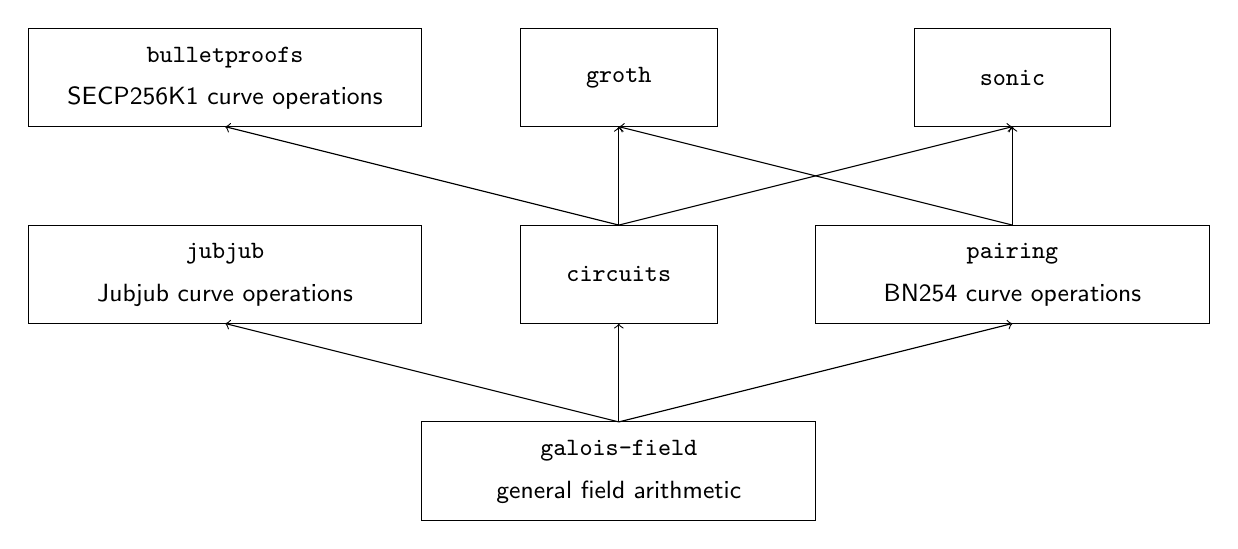
\begin{tikzpicture}[scale=1.25]
\draw (0, 0) rectangle node[above]{\small \texttt{galois-field}} node[below]{\small general field arithmetic} (4, 1);
\draw [->] (2, 1) to (-2, 2);
\draw [->] (2, 1) to (2, 2);
\draw [->] (2, 1) to (6, 2);
\draw (-4, 2) rectangle node[above]{\small \texttt{jubjub}} node[below]{\small Jubjub curve operations} (0, 3);
\draw (1, 2) rectangle node{\small \texttt{circuits}} (3, 3);
\draw [->] (2, 3) to (-2, 4);
\draw [->] (2, 3) to (2, 4);
\draw [->] (2, 3) to (6, 4);
\draw (4, 2) rectangle node[above]{\small \texttt{pairing}} node[below]{\small BN254 curve operations} (8, 3);
\draw [->] (6, 3) to (2, 4);
\draw [->] (6, 3) to (6, 4);
\draw (-4, 4) rectangle node[above]{\small \texttt{bulletproofs}} node[below]{\small SECP256K1 curve operations} (0, 5);
\draw (1, 4) rectangle node{\small \texttt{groth}} (3, 5);
\draw (5, 4) rectangle node{\small \texttt{sonic}} (7, 5);
\end{tikzpicture}
\end{center}

With the exception of minor discussions on design decisions, I was the primary developer of \texttt{galois-field} and the primary contributor to relevant functions in \texttt{semirings} and \texttt{poly}.

\pagebreak

\subsection{A universal library for elliptic curve operations}

Upon developing \texttt{galois-field} to a sufficiently flexible state, operations on the Jubjub curve were implemented in a single compact module under its own repository, to be used in a future protocol. Despite being an obvious next step, refactoring elliptic curve operations from \texttt{jubjub} and \texttt{pairing} was again not time-critical due to very minimal code duplication.

The realisation came soon after that the protocols under \texttt{groth} and \texttt{sonic} were designed over different elliptic curves in their respective papers. While \texttt{sonic} was meant to operate under a pairing algorithm designed for the \emph{BLS12-381} curve \cite{bls}, its implementation was missing from the stack, yet the protocol passed its functional tests under the pairing algorithm designed for \texttt{sonic}. This was borderline unsatisfactory, as unforeseen bugs may arise unexpectedly due to a potential lack of test coverage. Implementing BLS12-381 became the next course of action.

I proposed to transform the existing \texttt{jubjub} library into a universal library abstracting over all known elliptic curves used in Haskell cryptosystems. Due to the greater sophistication of elliptic curves, this would instead act as a database of elliptic curves domain parameters, in contrast to the functional library of Galois fields. This would overwrite existing internal implementations, so as to fully refactor primitives in the PBECC stack in the theme of separating concerns, and would also serve as a catalogue for future usages and references.

Upon agreement with the CTO, I started designing a hierarchy of type classes to emulate elliptic curves and their group of points, prioritising mathematical correctness and future extensibility over API cleanliness, as documentation would be sufficiently provided. An ideal hierarchy would encapsulate the various forms of elliptic curves, such as the usual Weierstrass form and the form given by Edwards curves, as well as the variability of the defining fields required in bilinear pairing computations. The initial design went along the following lines.
\begin{center}
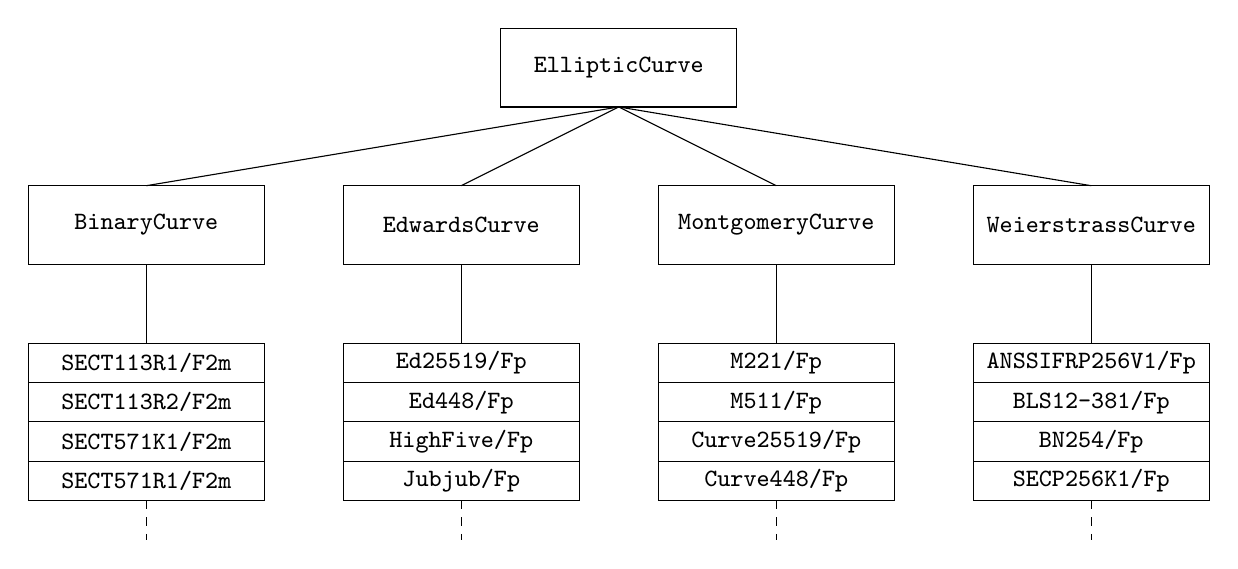
\begin{tikzpicture}
\draw (0, 0) rectangle node{\small \texttt{EllipticCurve}} (3, 1);
\draw (1.5, 0) to (-4.5, -1);
\draw (1.5, 0) to (-0.5, -1);
\draw (1.5, 0) to (3.5, -1);
\draw (1.5, 0) to (7.5, -1);
\draw (-6, -2) rectangle node{\small \texttt{BinaryCurve}} (-3, -1);
\draw (-4.5, -2) to (-4.5, -3);
\draw (-6, -3.5) rectangle node{\small \texttt{SECT113R1/F2m}} (-3, -3);
\draw (-6, -4) rectangle node{\small \texttt{SECT113R2/F2m}} (-3, -3.5);
\draw (-6, -4.5) rectangle node{\small \texttt{SECT571K1/F2m}} (-3, -4);
\draw (-6, -5) rectangle node{\small \texttt{SECT571R1/F2m}} (-3, -4.5);
\draw [dashed] (-4.5, -5) to (-4.5, -5.5);
\draw (-2, -2) rectangle node{\small \texttt{EdwardsCurve}} (1, -1);
\draw (-0.5, -2) to (-0.5, -3);
\draw (-2, -3.5) rectangle node{\small \texttt{Ed25519/Fp}} (1, -3);
\draw (-2, -4) rectangle node{\small \texttt{Ed448/Fp}} (1, -3.5);
\draw (-2, -4.5) rectangle node{\small \texttt{HighFive/Fp}} (1, -4);
\draw (-2, -5) rectangle node{\small \texttt{Jubjub/Fp}} (1, -4.5);
\draw [dashed] (-0.5, -5) to (-0.5, -5.5);
\draw (2, -2) rectangle node{\small \texttt{MontgomeryCurve}} (5, -1);
\draw (3.5, -2) to (3.5, -3);
\draw (2, -4.5) rectangle node{\small \texttt{Curve25519/Fp}} (5, -4);
\draw (2, -5) rectangle node{\small \texttt{Curve448/Fp}} (5, -4.5);
\draw (2, -3.5) rectangle node{\small \texttt{M221/Fp}} (5, -3);
\draw (2, -4) rectangle node{\small \texttt{M511/Fp}} (5, -3.5);
\draw [dashed] (3.5, -5) to (3.5, -5.5);
\draw (6, -2) rectangle node{\small \texttt{WeierstrassCurve}} (9, -1);
\draw (7.5, -2) to (7.5, -3);
\draw (6, -3.5) rectangle node{\small \texttt{ANSSIFRP256V1/Fp}} (9, -3);
\draw (6, -4) rectangle node{\small \texttt{BLS12-381/Fp}} (9, -3.5);
\draw (6, -4.5) rectangle node{\small \texttt{BN254/Fp}} (9, -4);
\draw (6, -5) rectangle node{\small \texttt{SECP256K1/Fp}} (9, -4.5);
\draw [dashed] (7.5, -5) to (7.5, -5.5);
\end{tikzpicture}
\end{center}
Here the classes involved would have two type parameters, one acting as a phantom parameter for the individual elliptic curve and the other being the Galois field defining the elliptic curve. For instance, the Jubjub curve would be represented with \texttt{EdwardsCurve Jubjub Fp}, an instance of the \texttt{class EdwardsCurve e k}, which is in turn a subclass of the general class.
\begin{verbatim}
    class GaloisField k => EllipticCurve e k
\end{verbatim}
Each of these classes would also have an associated data family representing the group of points, which would vary depending on the form of the elliptic curve.
\begin{verbatim}
    data family Point e k
\end{verbatim}
For instance, while usual elliptic curves have a distinguished \emph{point at infinity} \texttt{O} in addition to their \emph{affine points} \texttt{A k k}, the complete addition formula of Edwards curves remove the need for \texttt{O}, simplifying the control flow in point addition. A \texttt{Group} constraint was placed in the the definition of \texttt{EllipticCurve e k} to enforce the constraint in subclasses automatically.

Unfortunately, while simplistic in design, its implementation proved to be rather tricky in Haskell. In particular, the presence of gimmicks in the instance resolution system in Haskell, such as constraint erasure, made it difficult to properly mimic subclasses from object-oriented programming, while avoiding dangerous language extensions like \texttt{OverlappingInstances} and \texttt{AllowAmbiguousTypes}. For instance, since any \texttt{EdwardsCurve} $ E(K) $ is of the form
$$ E(K) = \{ (x, y) \in K^2 \mid Ax^2 + y^2 = 1 + Dx^2y^2 \}, \qquad A, D \in K, $$
it suffices to provide the $ K $-rational parameters $ A $ and $ D $ to specify the complete addition formula in \texttt{EllipticCurve}, yet it is fundamentally impossible to provide a default type class method, namely \texttt{add :: Point e k -> Point e k -> Point e k}, before supplying a complete set of information, namely the domain parameters specific to individual elliptic curves.

The heart of this problem lies in the inability to simultaneously define a constrained \texttt{class EllipticCurve e k => EdwardsCurve e k}, where the domain parameters would be taken in, as well as a default \texttt{instance EdwardsCurve e k => EllipticCurve e k}, where the addition formulas would be supplied. An obvious workaround to this issue could be to instead wrap the original phantom parameter in a \texttt{newtype EdwardsCurve e}, but this was quickly dismissed due to the troublesome multi-layered API it presents. It was only later when I realised that adding a new type parameter to \texttt{EllipticCurve e k}, which would represent the form of the elliptic curve, would solve this problem by allowing for both \texttt{class EllipticCurve 'Edwards e k => EdwardsCurve e k} and \texttt{instance EdwardsCurve e k => EllipticCurve 'Edwards e k} to be defined, albeit being slightly cumbersome. Subsequently, a new kind \texttt{Form}, with phantom constructors \texttt{Binary}, \texttt{Edwards}, \texttt{Montgomery}, and \texttt{Weierstrass}, representing the four relevant forms of elliptic curves, was added to give the following new class definition.
\begin{verbatim}
    class GaloisField k
        => EllipticCurve (f :: Form) e k where
        data family Point f e k :: *
\end{verbatim}

With a newfound realisation for additional type parameters, at least two notable feature additions were then made accessible. The first of these allowed for a transformation of coordinate systems, from the default \texttt{Affine} coordinates to \texttt{Projective} and \texttt{Jacobian} coordinates, all encoded as phantom constructors under a new kind \texttt{Coordinates}. While making the entire library more flexible, new coordinate systems also allowed for experimental performance comparisons. For instance, I discovered that \texttt{Projective} coordinates, which have a longer multiplication formula but no divisions, were significantly faster for an \texttt{EdwardsCurve}, but \texttt{Affine} coordinates were sufficient for all other elliptic curves. The class definition then became the following.
\begin{verbatim}
    class GaloisField k
        => EllipticCurve (f :: Form) (c :: Coordinates) e k where
        data family Point f c e k :: *
\end{verbatim}

The second addition was more technical and allowed for point multiplication to depend on the \emph{scalar prime field} of the elliptic curve, the Galois field of order equal to the subgroup order. This subgroup order would then be safely encoded in the type level, allowing for huge point multiplications to be bounded above. The class definition then became the following.
\begin{verbatim}
    class (GaloisField k, PrimeField n)
        => EllipticCurve (f :: Form) (c :: Coordinates) e k n where
        data family Point f c e k n :: *
\end{verbatim}

It remained to produce concrete elliptic curve implementations under this robust class design, with parameters collected from existing cryptosystems available across many online databases. These would include the elliptic curves used in internal libraries, namely BLS12-381, BN254, SECP256K1, and Jubjub, as well as the recommended elliptic curves by NIST \cite{sec2} and SafeCurves \cite{safecurves}. Due to a serious lack of canonical references and test vectors, their domain parameters were highly susceptible to typographic errors in online drafts. Fortunately, these were detected automatically by adding curve-invariant tests based around the \emph{discriminant} and the \emph{Hasse-Minkowski theorem}. In addition to these tests, the axioms of an abelian group were also verified given random points on a fixed elliptic curve. However, obtaining the notion of randomness required taking modular square roots in its defining field, say in the computation of $ y = \sqrt{x^3 + Ax + B} $ given a random field element $ x $, which was only implemented later. This arduous process of collecting data and verifying correctness took at least two weeks.

During development, due to the sheer number of elliptic curve modules, I also added a simple Haskell source code generator, which originally served as a gadget to hasten data collection and automate testing. This was later developed sufficiently as a standalone project in the same repository to allow for effortless long-term maintenance and possibly future contributions.

After a total period of five weeks, the end result was a large library of eighty elliptic curves used in common cryptosystems, now published on Hackage as \texttt{elliptic-curve} \cite{elliptic-curve}. This was again equipped with sufficiently detailed documentation to add new forms or coordinates of elliptic curves, making the library easily extensible by public contributions. The elliptic curves in existing internal libraries were subsequently replaced with a dependency on \texttt{elliptic-curve}, giving the following new PBECC stack layout.
\begin{center}
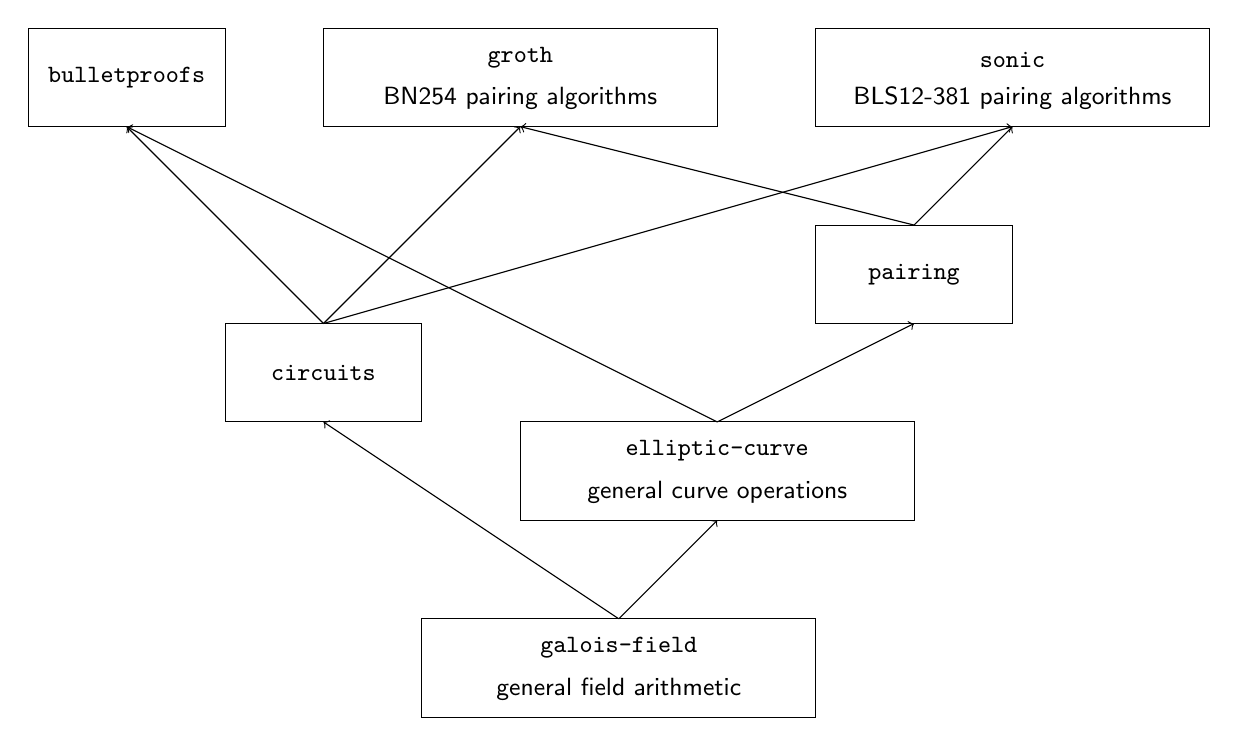
\begin{tikzpicture}[scale=1.25]
\draw (0, 0) rectangle node[above]{\small \texttt{galois-field}} node[below]{\small general field arithmetic} (4, 1);
\draw [->] (2, 1) to (-1, 3);
\draw [->] (2, 1) to (3, 2);
\draw (-2, 3) rectangle node{\small \texttt{circuits}} (0, 4);
\draw [->] (-1, 4) to (-3, 6);
\draw [->] (-1, 4) to (1, 6);
\draw [->] (-1, 4) to (6, 6);
\draw (1, 2) rectangle node[above]{\small \texttt{elliptic-curve}} node[below]{\small general curve operations} (5, 3);
\draw [->] (3, 3) to (-3, 6);
\draw [->] (3, 3) to (5, 4);
\draw (4, 4) rectangle node{\small \texttt{pairing}} (6, 5);
\draw [->] (5, 5) to (1, 6);
\draw [->] (5, 5) to (6, 6);
\draw (-4, 6) rectangle node{\small \texttt{bulletproofs}} (-2, 7);
\draw (-1, 6) rectangle node[above]{\small \texttt{groth}} node[below]{\small BN254 pairing algorithms} (3, 7);
\draw (4, 6) rectangle node[above]{\small \texttt{sonic}} node[below]{\small BLS12-381 pairing algorithms} (8, 7);
\end{tikzpicture}
\end{center}

I was the primary developer of \texttt{elliptic-curve}, but I had many consultations with a colleague on the general type system of Haskell throughout the initial class design.

\pagebreak

\subsection{A polymorphic library for bilinear pairing algorithms}

The development of BLS12-381 in \texttt{elliptic-curve} was ultimately a bridge for a bilinear pairing algorithm suitable for the \texttt{sonic} protocol. However, after spending a week internalising the complex algorithm by consulting online resources, while refactoring several now redundant functions such as complex conjugation and Frobenius endomorphisms, I realised that the existing algorithm in \texttt{pairing} was tailored too specifically for BN254. In particular, branching out to account for a new elliptic curve was not directly possible.

I proposed a clean rewrite of the existing \emph{optimal ate pairing} algorithm \cite{beuchat} to be polymorphic over BLS12-381 and BN254, which would provide the expected bilinear pairing algorithm for the \texttt{sonic} protocol, although the final result came to be quite different. As the existing code was based on an external library written in C and had a procedural style in its execution, I suggested for a rewrite in a declarative style more comprehensible in Haskell, which could be refactored more easily if the need ever arises in the future.

Upon agreement with the CTO, my first course of action was to write a generic class to contain the type class method for bilinear pairings of general cryptographic groups.
\begin{verbatim}
    class (Group (G1 e), Group (G2 e), Group (GT e))
        => Pairing e where
        type G1 e = (g1 :: *) | g1 -> e
        type G2 e = (g2 :: *) | g2 -> e
        type GT e = (gt :: *) | gt -> e
        pairing :: G1 e -> G2 e -> GT e
\end{verbatim}
Here the single phantom parameter would encode the two choices of elliptic curves, namely BLS12-381 and BN254. The three associated types would denote the left, right, and target groups respectively, with explicit injective annotations to unambiguously define \texttt{pairing}, a function replacing the existing \texttt{reducedPairing :: G1 BN254 -> G2 BN254 -> GT BN254}. There were several drastic changes to this class definition over the following weeks to account for compatibility, but I eventually returned to this initial design.

The majority of the remaining time was spent on implementing the actual algorithm, which was supplemented with pre-written QuickCheck tests and Criterion benchmarks to ensure constant improvement over the old algorithm. As per the case for general elliptic curves, there were no canonical references available online on the exact pairing parameters, so debugging the minuscule errors that accumulated over the lengthy algorithm took a very long time. In particular, the tricky \texttt{lineFunction :: G2 e -> G2 e -> G1 e -> GT e -> GT e}, which was fundamental to the algorithm, had an unexpected type definition and was very difficult to implement, taking up to two weeks to fully debug with external test vectors.

While the exact details of the implementation will be omitted here for brevity, the algorithm itself could be split into two distinct parts, namely a \emph{Miller algorithm} and a \emph{final exponentiation}. The former involves a lengthy loop of point additions and line functions, but the loop itself could be significantly shortened depending on the decomposition of an curve-dependent integer into signed binary digits. The latter is a simple exponentiation operation in a large Galois field that took up the majority of the computation time, but this could again be decomposed into several much smaller exponentiations. While the old implementation did not allow for both of these optimisations, the new abstraction made it almost trivial to do them. At the presence of fair benchmarks, there was a significant speedup by a factor of two to three compared to the original algorithm, which already had a noticeable computation time in the millsecond range.

Surprisingly, due to this clean abstraction, the library could be made polymorphic over even more elliptic curves. In particular, both BLS12-381 and BN254 exhibit a \emph{four-tower extension field} system, a property very common amongst pairing-friendly elliptic curves. The newly abstracted optimal ate pairing algorithm could then be made polymorphic over all of these elliptic curve families, and a five more elliptic curves were added to establish this proof of concept, although it is easy to add more when the need arises.

Furthermore, there was already an existing hashing algorithm in \texttt{pairing} based on the simple \emph{Shallue-von de Woestijne encoding} \cite{fouque}, which was completely separate from the main pairing functionality. This was originally added by a public contributor and worked only for BN254, so I simply rewrote it, with existing functions from \texttt{galois-field} in mind, to allow polymorphism over the remaining elliptic curves. Again, in a delightful surprise, the newly abstracted algorithm was hundreds of times faster than the old algorithm.

After a total period of four weeks, the end result was a polymorphic pairing class over seven proof-of-concept elliptic curves, now published in a new version on Hackage as \texttt{pairing} \cite{pairing}. As there was already existing documentation in the landing page, I added some further documentation to explain several optimisation decisions I made throughout the algorithm, as well as some potential optimisations I did not add due to lack of time. Finally, a minor refactoring of \texttt{sonic} to depend on the BLS12-381 pairing gave the following PBECC stack layout.
\begin{center}
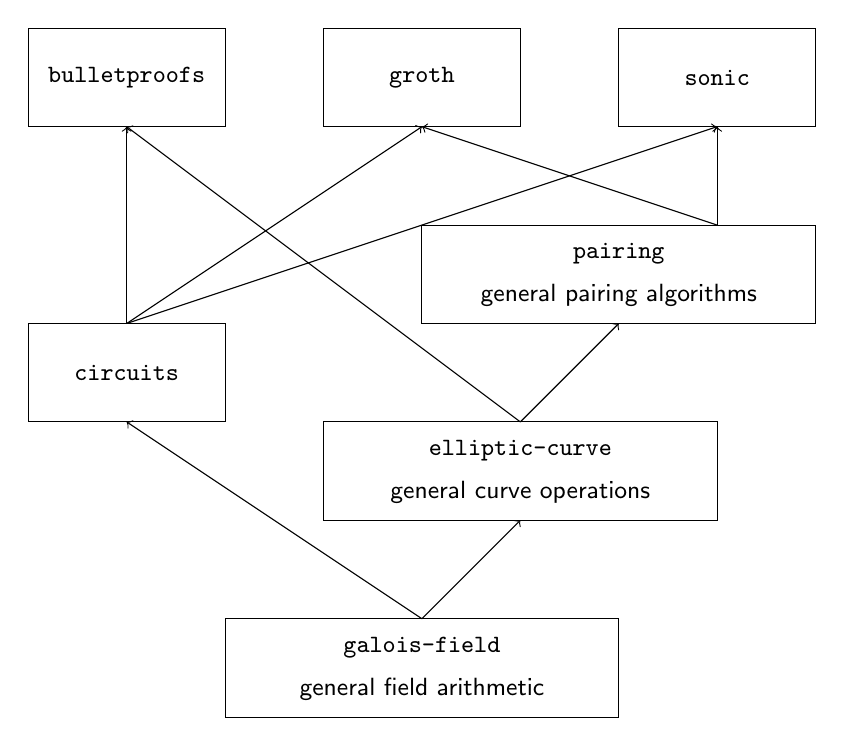
\begin{tikzpicture}[scale=1.25]
\draw (0, 0) rectangle node[above]{\small \texttt{galois-field}} node[below]{\small general field arithmetic} (4, 1);
\draw [->] (2, 1) to (-1, 3);
\draw [->] (2, 1) to (3, 2);
\draw (-2, 3) rectangle node{\small \texttt{circuits}} (0, 4);
\draw [->] (-1, 4) to (-1, 6);
\draw [->] (-1, 4) to (2, 6);
\draw [->] (-1, 4) to (5, 6);
\draw (1, 2) rectangle node[above]{\small \texttt{elliptic-curve}} node[below]{\small general curve operations} (5, 3);
\draw [->] (3, 3) to (-1, 6);
\draw [->] (3, 3) to (4, 4);
\draw (2, 4) rectangle node[above]{\small \texttt{pairing}} node[below]{\small general pairing algorithms} (6, 5);
\draw [->] (5, 5) to (2, 6);
\draw [->] (5, 5) to (5, 6);
\draw (-2, 6) rectangle node{\small \texttt{bulletproofs}} (0, 7);
\draw (1, 6) rectangle node{\small \texttt{groth}} (3, 7);
\draw (4, 6) rectangle node{\small \texttt{sonic}} (6, 7);
\end{tikzpicture}
\end{center}

With the exception of frequent Haskell consultations, I was again the primary developer of the new \texttt{pairing} library, but I was assisted by a colleague during some of its initial changes to account for \texttt{galois-field} and \texttt{elliptic-curve}. This project served as a closure to the primitive-level restructuring of the PBECC stack, but it is only my wish to maintain it further. For instance, the next step would be to make \texttt{pairing} polymorphic over all pairing-friendly elliptic curve families, rather than merely those with a four-tower extension field system.

\pagebreak

\section{Conclusion}

I thoroughly enjoyed my experience throughout my industrial placement in Adjoint over the course of seventeen weeks, and hope to return as a full-time employee upon graduation.

\subsection{Courses relevance}

Working towards a degree in Mathematics and Computer Science in Imperial certainly made this enjoyment possible. At the most basic level, the various skills I picked up in numerous laboratory exercises and projects, including communicative collaboration, productivity management, and general software engineering practices, made it possible to deliver prototypical libraries in allocated time periods. Having several lectures on presentation skills and professional ethics also allowed me to convey my thoughts rationally in several talks I gave in my final weeks.

At a more technical level, there were several courses in the Department of Computing where, without having a firm foundation in these, such an experience would be highly unlikely. The most crucial of these is the first year Haskell course, where I was first exposed to the basics of the language. This was further supplemented with the advanced programming lectures, where I was first exposed to more fundamental concepts like type-level programming. The fascination I had in the first year led me to study Haskell at a deeper level in later years. With a sufficient proficiency in Haskell, I was then able to write code of demonstrable quality right away, as well as rapidly understanding further technicalities in the type system along the way.

In contrast, the courses in the Department of Mathematics played a far bigger role in allowing me to constantly produce deliverables in the form of mathematical libraries. These include the various algebra and number theory courses over four years, particularly the fourth year elliptic curves and algebraic geometry courses. This was further complemented with my second year summer research project on the arithmetic of elliptic curves, where I also learnt to pick up important pieces of information in technical papers outside my domain of knowledge. Having a firm foundation in basic algebra and number theory allowed me to process my thoughts abstractly and write mathematically accurate code confidently without referring to any resources.

\subsection{Useful skills}

On the other hand, I would have been much more productive in the early stages of my projects if I had prior exposure in contributing to medium-sized open source repositories in Haskell. For instance, it took unnecessarily long to internalise the existing implementations of bilinear pairings and arithmetic circuits, which could be avoided with further experience in Haskell. A better familiarity with common libraries, such as QuickCheck and Criterion, would have been wonderful, especially in the development of functional libraries like \texttt{galois-field} where performance is crucial. For instance, this would have prevented inaccurate performance benchmarks using \texttt{whnf} rather than \texttt{nf} for normal form evaluation in a cheap computation.

It would have also been more convenient to have a higher proficiency in type-level Haskell from the get go. For instance, there were certain tricks or quirks I was completely unaware of, such as using type equalities to avoid ambiguity, or the weird behaviour of the instance resolution system that I thought was bugged. Some of these forced me to come up with inelegant workarounds that were eventually replaced. It is unfortunate that Haskell is greatly downplayed in my degree, but having a firm foundation in mathematical abstraction made it easy to absorb new concepts introduced to me. Moreover, I had a wonderful colleague who I consulted frequently with throughout my journey in Haskell.

Furthermore, it would have been beneficial to better understand the underpinnings of contemporary cryptography from the get go. Although the mathematics behind PBECC was easy, I was not aware of the existence of such applications and had no chance of studying them prior to the industrial placement, which delayed my implementation of cryptographic protocols like \texttt{groth}. As such, despite implementing an initial prototype in the first weeks, I did not understand its use cases until it was actually deployed as part of a larger system.

\subsection{Personal benefits}

On the other hand, the seventeen weeks of hard work was fortunately worth the weight. As this was my first external paid internship, I was exposed to the various ups and downs of modern industry. This was an entirely different experience in contrast to the academic world I longed to stay in, which changed my perspective of the industrial world, mostly in a good way.

At a more technical level, I recognised the applicability of my knowledge and the extent of my limitations, and was driven to further understand Haskell and cryptography. After developing several libraries, I also realised the importance of dependency management and version control, especially when two libraries inexplicably depend on one another.

Furthermore, I internalised the various concepts introduced to me over the industrial placement. In particular, these included the theory of Petri nets and graph unfolding algorithms in my short research on \texttt{fcl}, as well as the theory behind quadratic arithmetic programs and zero-knowledge proofs required in the understanding of \texttt{groth}.

\subsection{Ethical considerations}

My wonderful experience was also complemented with great professional conduct from my colleagues. Despite coming from various cultural backgrounds, a great deal of mutual respect is displayed during all of our interactions, be it during work or outside of work, and there were never any obligation to reveal personal issues that may violate privacy of an individual.

In my first weeks, I was given ample time to understand the relevant theory in the domain as well as the code in existing repositories, without a feeling of incompetence. In the later weeks, I have always received technical and moral support throughout the development of the various libraries, which allowed me to finish my tasks readily but enjoyably.

Most of the existing repositories were equipped with documentation that had clear acknowledgements to external references, be it in the readme or as inline comments. This would give credit to all contributors of knowledge, but there were instances where code contributors were not given enough credit, especially when a large pool of commits was squashed before merging.

\pagebreak

\begin{thebibliography}{20}

\bibitem{adjoint}
Adjoint UK Ltd. \texttt{adjoint.io}

\bibitem{treasury}
Adjoint UK Ltd. \emph{Treasury}. \texttt{adjoint.io/product}

\bibitem{uplink}
Adjoint UK Ltd. \emph{Uplink}. \texttt{adjoint.io/technology}

\bibitem{fcl}
Adjoint UK Ltd. \emph{FCL}. \texttt{github.com/adjoint-io/fcl}

\bibitem{cryptography}
Adjoint UK Ltd. \emph{Upperlink}. \texttt{dev.adjoint.io/crypto.html}

\bibitem{bulletproofs}
Adjoint UK Ltd. \emph{Bulletproofs}. \texttt{hackage.haskell.org/package/bulletproofs}

\bibitem{sonic}
Adjoint UK Ltd. \emph{Sonic}. \texttt{github.com/adjoint-io/sonic}

\bibitem{galois-field}
Adjoint UK Ltd. \emph{Galois fields}. \texttt{hackage.haskell.org/package/galois-field}

\bibitem{elliptic-curve}
Adjoint UK Ltd. \emph{Elliptic curves}. \texttt{hackage.haskell.org/package/elliptic-curve}

\bibitem{pairing}
Adjoint UK Ltd. \emph{Bilinear pairings}. \texttt{hackage.haskell.org/package/pairing}

\bibitem{semirings}
chessai. \emph{Semirings}. \texttt{hackage.haskell.org/package/semirings}

\bibitem{poly}
Bodigrim. \emph{Polynomials}. \texttt{hackage.haskell.org/package/poly}

\bibitem{kostin}
A E Kostin, 2006. \emph{A Reachability Algorithm for General Petri Nets Based on Transition Invariants}. \texttt{researchgate.net/publication/225237686\_A\_Reachability\_Algorithm} \\
\texttt{\_for\_General\_Petri\_Nets\_Based\_on\_Transition\_Invariants}

\bibitem{mcmillan}
J Esparza et al, 2002. \emph{An Improvement of McMillan's Unfolding Algorithm}. \\
\texttt{researchgate.net/publication/225898331\_An\_Improvement\_of} \\
\texttt{\_McMillan's\_Unfolding\_Algorithm}

\bibitem{groth}
J Groth, 2016. \emph{On the Size of Pairing-based Non-interactive Arguments}. \\ \texttt{eprint.iacr.org/2016/260.pdf}

\bibitem{qap}
V Buterin, 2016. \emph{Quadratic Arithmetic Programs: from Zero to Hero}. \\ \texttt{medium.com/@VitalikButerin/quadratic-arithmetic-programs} \\ \texttt{-from-zero-to-hero-f6d558cea649}

\bibitem{jubjub}
ZCash. \emph{What is Jubjub?}.
\texttt{z.cash/technology/jubjub}

\bibitem{bls}
Electric Coin Company. \emph{BLS12-381: New zk-SNARK Elliptic Curve Construction}. \\
\texttt{electriccoin.co/blog/new-snark-curve}

\bibitem{sec2}
Certicom Research, 2000. \emph{SEC2: Recommended Elliptic Curve Domain Parameters}. \\
\texttt{secg.org/SEC2-Ver-1.0.pdf}

\bibitem{safecurves}
D J Bernstein et al. \emph{SafeCurves: Choosing Safe Curves for Elliptic-Curve Cryptography}. \\
\texttt{safecurves.cr.yp.to}

\bibitem{beuchat}
J L Beuchat et al, 2010. \emph{High-Speed Software Implementation of the Optimal Ate Pairing over Barreto–Naehrig Curves}. \texttt{eprint.iacr.org/2010/354.pdf}

\bibitem{fouque}
P A Fouque et al, 2012. \emph{Indifferentiable Hashing to Barreto–Naehrig Curves}. \\
\texttt{di.ens.fr/~fouque/pub/latincrypt12.pdf}

\end{thebibliography}

\end{document}